\documentclass[11pt]{article}

\usepackage[margin=1in]{geometry}
\usepackage[T1]{fontenc}
\usepackage[utf8]{inputenc}
\usepackage{lmodern}
\usepackage{graphicx}
\usepackage{booktabs,array}
\usepackage[nointegrals]{wasysym}
\usepackage[numbers,sort&compress]{natbib}
\usepackage[hidelinks]{hyperref}
\usepackage[labelfont=bf,labelsep=period]{caption}
\newcommand{\botrule}{\bottomrule}
\providecommand{\bibcommenthead}{}

\begin{document}

\begin{center}
{\Large\bfseries Additional file 1}\\[0.6em]
{\large PoolParty: streamlined design of DNA sequence libraries in Python}\\[0.8em]
{\large Supplementary methods, figures, and tables}
\end{center}

\section*{Supplementary Methods}

Benchmarks were run under Ubuntu 22.04.3 LTS in Windows Subsystem for Linux 2
on an Intel Core Ultra 9 185H workstation with 31~GB RAM allocated to WSL2,
using CPython 3.12.2, PoolParty 0.1.0, and StateTracker 0.1.0. Timings are
single-threaded wall-clock measurements of \texttt{generate\_library}, reported
as mean $\pm$ SD over five replicate runs. Peak memory is the maximum resident
set size reported by \texttt{getrusage}, with each data point measured in a
fresh process.

\renewcommand{\thefigure}{S\arabic{figure}}
\renewcommand{\thetable}{S\arabic{table}}
\renewcommand{\theHfigure}{S\arabic{figure}}
\renewcommand{\theHtable}{S\arabic{table}}
\setcounter{figure}{0}
\setcounter{table}{0}

\begin{figure}[p]
\centering
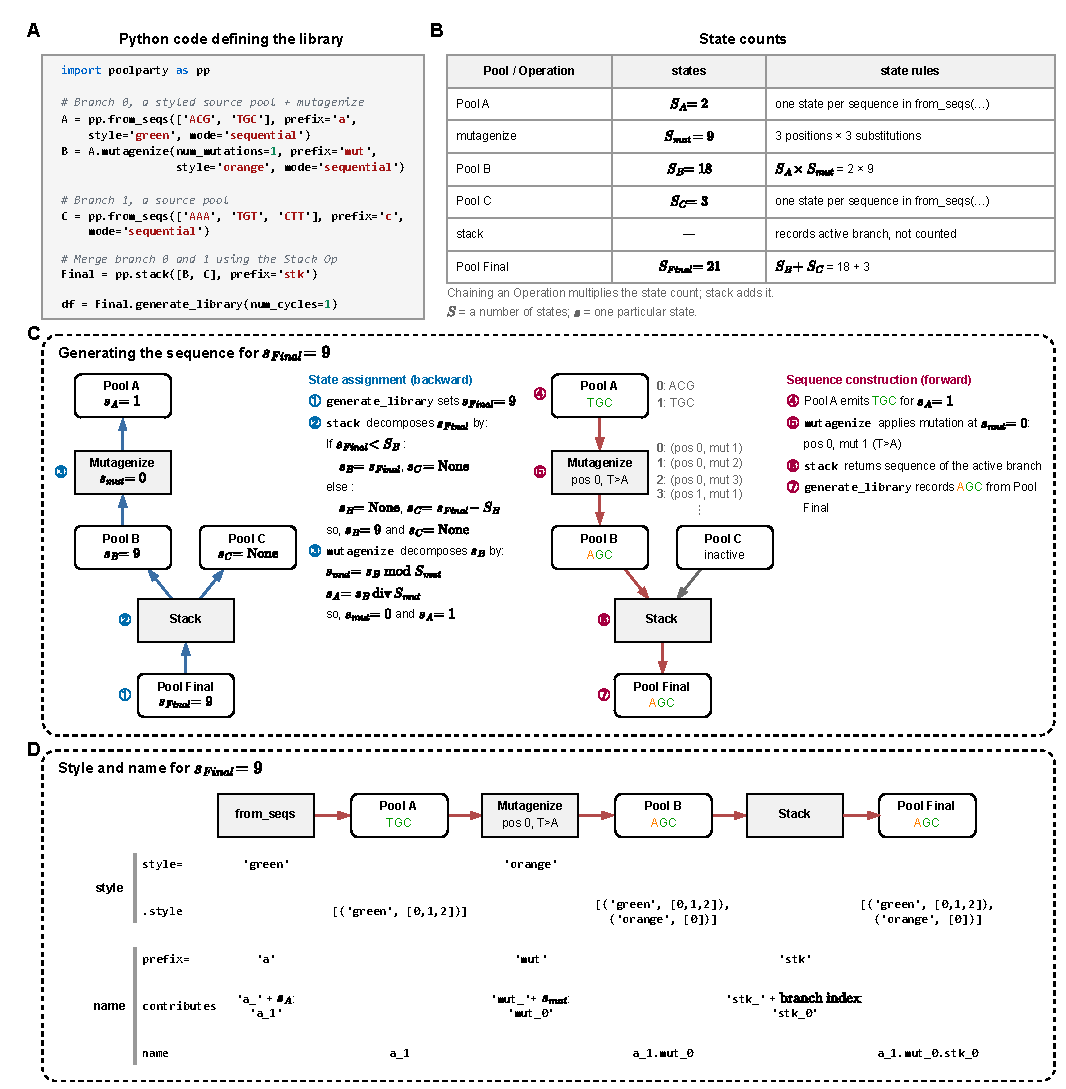
\includegraphics[width=\textwidth]{assets/figure_s1_sequence_generation}
\caption{\textbf{A worked example of sequence generation.}
\textbf{(A)} Python code defining the DAG in Fig.~1B of the main text.
\textbf{(B)} Number of states of each Pool and Operation.
\textbf{(C)} Generating the sequence for $s_{Final} = 9$. Left: state assignment
(blue). Right: sequence construction (magenta). Lists beside Pool A and
\texttt{mutagenize} show which sequence or mutation each state selects. Inactive
branches are shown in grey. \textbf{(D)} Style and name for the same sequence.
Sequences are carried through the DAG as \texttt{Seq} objects, which hold the
sequence string together with its \texttt{.style}. The \texttt{style} and
\texttt{prefix} arguments are supplied to Operations; the resulting
\texttt{.style} and name are held by Pools. Sequence characters are colored by
their \texttt{.style} entries; where entries overlap, the last one applies.
The styling shown in Panel D was generated by setting \texttt{\_include\_inline\_styles=True} in \texttt{Final.generate\_library()}; this is omitted from the code snippet in panel A.}
\label{fig:sequence-generation}
\end{figure}

\begin{figure}[p]
\centering
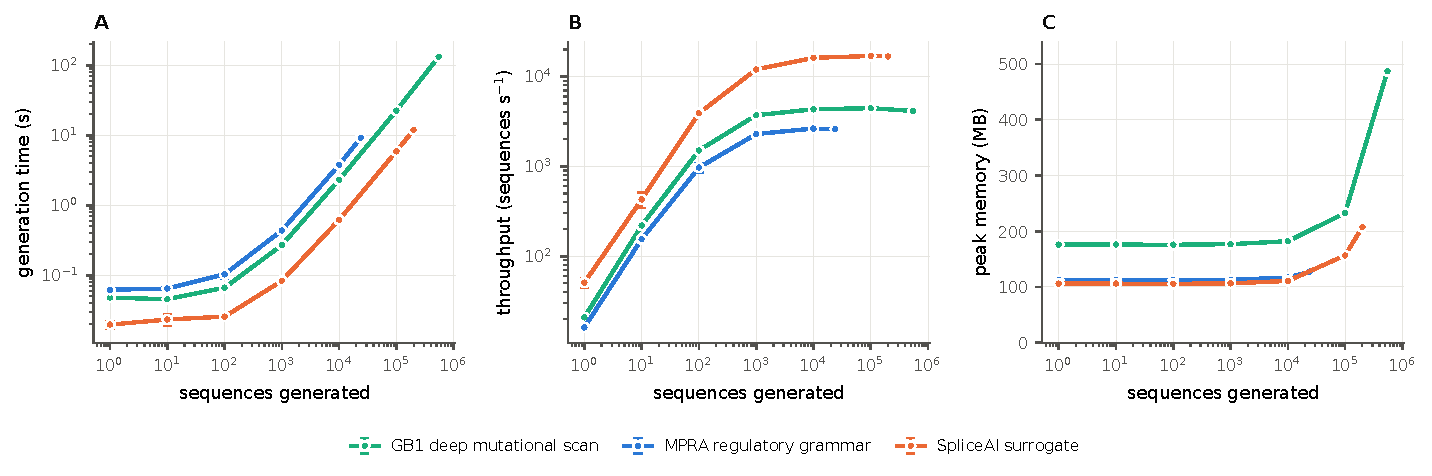
\includegraphics[width=\textwidth]{assets/figure_s2_benchmark_scaling}
\caption{\textbf{Library generation scales linearly in time and memory.}
\textbf{(A)} Wall-clock generation time, \textbf{(B)} throughput, and
\textbf{(C)} peak resident memory against the number of sequences generated, for
the three worked examples. Points are means of 5 replicate runs; error bars show
$\pm$1~SD and are smaller than the plotting symbols at most points. Below
$\sim$10$^3$ sequences a fixed setup cost dominates, giving the plateau in
\textbf{(A)} and the rise in \textbf{(B)}; above 10$^4$ sequences throughput is
constant, so generation time is linear in library size. Peak memory increases
linearly, by 0.52--0.66~kB per sequence above a $\sim$106~MB baseline for the MPRA and SpliceAI libraries; similar behavior is observed for the GB1 library, but with a higher memory baseline.}
\label{fig:benchmark-scaling}
\end{figure}

\begin{figure}[p]
\centering
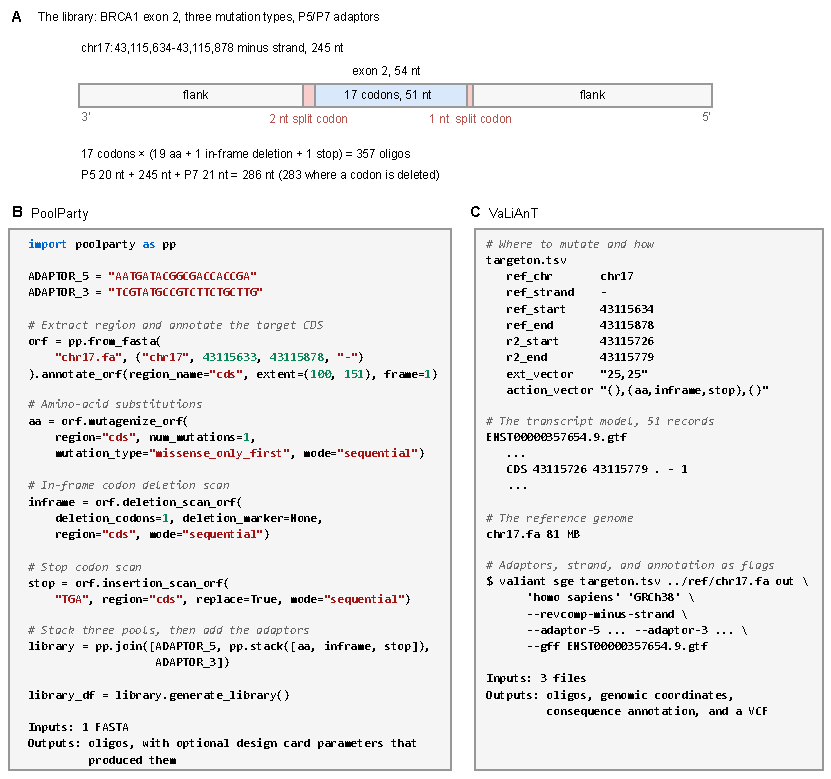
\includegraphics[width=\textwidth]{assets/figure_s3_valiant_comparison}
\caption{\textbf{The same BRCA1 exon 2 variant library in PoolParty and
VaLiAnT.} \textbf{(A)} For each of the 17 complete codons in BRCA1 exon 2, the
library contains substitutions to the other 19 amino acids, one stop-codon
substitution, and one in-frame codon deletion. This gives 357 oligos. The split
codons at the exon boundaries are left unchanged, and P5 and P7 adaptors are
added to each sequence. \textbf{(B)} PoolParty implementation. The reference
sequence is loaded from a FASTA file, and the user supplies the extent and
reading frame of the 17 complete codons. Three ORF-aware Operations generate the
amino-acid, stop-codon, and deletion scans. \textbf{(C)} VaLiAnT 4.0.0
implementation. VaLiAnT takes a coordinate and action table, a GTF annotation,
and the reference chromosome as input. VaLiAnT gets the CDS phase from the GTF;
in PoolParty, the user supplies the ORF extent and frame. The PoolParty code
additionally calls
\texttt{pp.set\_genetic\_code(valiant\_codon\_preference())} to match VaLiAnT's
arginine codon choice; this setup line is omitted from panel B. When configured
to use the same codon usage table, PoolParty and VaLiAnT gave exactly the same
set of 357 sequences.}
\label{fig:valiant-comparison}
\end{figure}

\begin{figure}[p]
\centering
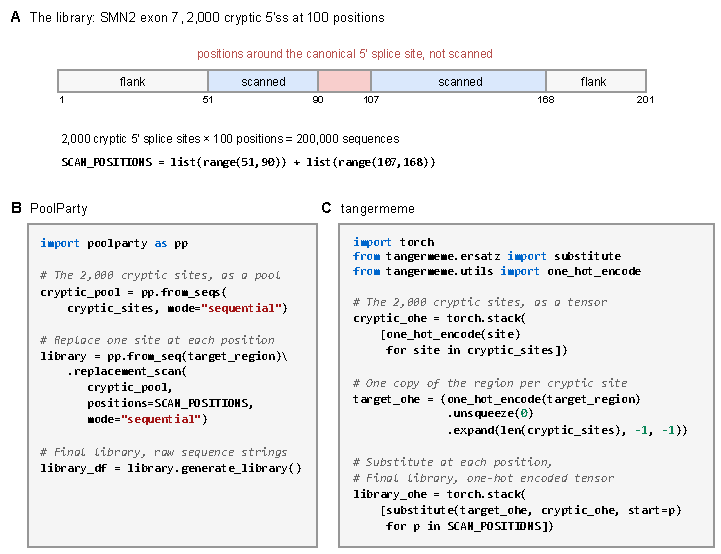
\includegraphics[width=\textwidth]{assets/figure_s4_tangermeme_comparison}
\caption{\textbf{The same cryptic splice-site perturbation library in PoolParty
and tangermeme.} \textbf{(A)} The library contains 2,000 cryptic 5$'$ss 9-mers,
each substituted at 100 positions across a 201-bp region containing the
canonical 5$'$ss of SMN2 exon 7, giving 200,000 sequences. Positions immediately
around the canonical site are excluded. This is the GT arm of the library in
main-text Fig.~4; the matched control arm is built the same way.
\textbf{(B)} PoolParty implementation. The 2,000 sites form a Pool, and
\texttt{replacement\_scan} substitutes them at the 100 positions. The generated
sequences are returned as strings in a table. \textbf{(C)} tangermeme 1.4.1
implementation. The target region and cryptic sites are one-hot encoded,
substitutions are applied in one batch per position, and the final output is a
tensor. After decoding this tensor, the two implementations gave the same set of
200,000 sequences.}
\label{fig:tangermeme-comparison}
\end{figure}

\begin{table}[p]
\centering
\footnotesize
\caption{\textbf{Runtime and memory for the three worked examples.} Each example
was generated at the size shown using a single core. Generation times are means
$\pm$ SD over five replicate runs. Peak memory is maximum resident set size and
includes the fixed memory used by Python and the example DAG. DAG construction
does not depend on library size and is reported separately. The SpliceAI
library comprises two matched 200,000-sequence pools (cryptic GT and disrupted
GA) generated separately; values are for one pool, and the full library takes
twice as long.}
\label{tab:benchmark-summary}
\begin{tabular}{@{}lrrrrr@{}}
\toprule
Example & Library size & Time (s) & Sequence/s & Memory (MB) & DAG (s)\\
\midrule
GB1 deep mutational scan & 547,230 & $132.24 \pm 5.76$ & 4,138 & 487 & 0.22\\
MPRA regulatory grammar & 24,000 & $9.22 \pm 0.22$ & 2,602 & 127 & 0.06\\
SpliceAI surrogate & 200,000 & $11.93 \pm 0.27$ & 16,758 & 208 & 0.05\\
\botrule
\end{tabular}
\end{table}

% Supplementary tool overview. This file is the rendered deliverable;
% design decisions are recorded in table1.md.
% Requires: booktabs, array
% Individually listed tools are alphabetical; two grouped rows follow.
% PoolParty is bold, not first.
\begin{table}[tbp]
\centering
\scriptsize
% (setspace override omitted: measured to have no effect inside this float)
\setlength{\tabcolsep}{3pt}
\renewcommand{\arraystretch}{0.9}
\caption{\textbf{Tools for designing DNA sequence libraries and for
related sequence-design problems.} The final two rows group related tools; their
members are named and cited individually.}
\label{tab:tools}
\begin{tabular}{@{}>{\raggedright\arraybackslash}p{2.0cm}>{\raggedright\arraybackslash}p{3.4cm}>{\raggedright\arraybackslash}p{4.3cm}>{\raggedright\arraybackslash}p{2.15cm}@{}}
\toprule
\textbf{Tool} & \textbf{Purpose / availability} & \textbf{Key features} &
\textbf{Output}\\
\midrule

MPRA Design Tools \citep{Ghazi2018aa} &
Design MPRA libraries and estimate statistical power. R package (GitHub). &
Barcode assignment with error-correcting sets; power analysis over effect
size and sequencing depth &
Barcoded constructs and statistical power estimates\\
\addlinespace

MPRAnator \citep{GeorgakopoulosSoares2017gb} &
Design MPRA libraries of motif arrangements and sequence variants. Web
service. &
Combinatorial placement of motifs; randomly sampled and combinatorial
substitution sets; scrambled and reverse-complement controls &
Barcoded library of sequences (FASTA)\\
\addlinespace

Mutation Maker \citep{Hiraga2021yg} &
Design mutagenic oligos for building variant libraries in the laboratory.
Web application (Docker); REST API. &
Degenerate codons at user-listed sites; several substitutions combined in
one reaction; de novo gene assembly with per-site variant frequencies &
Primers, or gene fragments with the proportion of each variant to pool\\
\addlinespace

Oligopool Calculator \citep{Hossain2024oc} &
Add barcodes, primers, and spacers to a supplied variant set, and analyze
the sequencing readout. Python package (PyPI); command line. &
Constraint-aware barcodes, primers, and spacers; degenerate compression of
a supplied variant set; off-target screening against a host genome &
Synthesis-ready constructs; variant counts from sequencing reads\\
\addlinespace

\textbf{PoolParty} &
Design libraries that combine multiple variant types for laboratory assays
or for probing genomic AI models. Python package (PyPI). &
Libraries specified as a directed acyclic graph of Operations, allowing
different mutagenesis schemes to be combined; sequences generated only on
request &
Library of sequences, each paired with a record of how it was constructed\\
\addlinespace

tangermeme \citep{Schreiber2025nd} &
Generate perturbed sequence sets to probe cis-regulatory logic in deep
learning models. Python package (PyPI). &
Saturation mutagenesis of input sequences; insertion and removal of motifs
across sets of sequences &
Perturbed sequences, model predictions, or attribution scores\\
\addlinespace

VaLiAnT \citep{Barbon2022th} &
Design and annotate libraries for saturation genome editing and cDNA deep
mutational scanning. Command-line tool (source, Docker). &
Saturation mutagenesis from genomic coordinates; several mutation types
per target region; transcript-aware, including codons split across exons &
Per-region libraries with metadata tables and VCF carrying variant
consequence annotation\\
\midrule

General-purpose toolkits\newline\textit{(Biopython, pydna, SeqPro)} \citep{Cock2009df,Pereira2015wj,Klie2023kg} &
Manipulate sequences, simulate cloning, prepare arrays for modeling.
Python packages (PyPI). &
Parsing, transformation, and file-format support &
Transformed sequences\\
\addlinespace

Sequence optimization tools\newline\textit{(CodonGenie, DNA Chisel, ledidi)} \citep{Swainston2017rb,Zulkower2020jk,Schreiber2025ledidi} &
Optimize individual sequences for codon usage, synthesis constraints, or a
model's objective. Python packages (PyPI); web services. &
Degenerate codons covering a target residue set; hard constraints and
scored objectives combined in one problem; gradient-based editing guided
by a predictive model &
An optimized or edited sequence, or a degenerate codon\\
\botrule
\end{tabular}
\end{table}

\input{assets/table_s3_capabilities}

\clearpage
\bibliographystyle{sn-vancouver-num}
\bibliography{references}

\end{document}
